\documentclass[../main-v1.tex]{subfiles}
\begin{document}
\chapter{Code Management \hideme{Tom Junk, Mathew Muether, David Adams - draft}}
\label{ch:codemgmt}

%%%%%%%%%%%%%%%%%%%%%%%%%%%%%%%%
\section{Liquid Argon TPC Code Management \hideme{Junk/Calcutt - needs update}}
\label{sec:codemgmt:dunetpc}  %% fix label according to section

Software for simulation, data read-in, and reconstruction shares significant commonality across the liquid-argon time projection chamber detectors planned to be deployed by DUNE and also prototypes.  These comprise the 35-ton prototype, ProtoDUNE-SP, ProtoDUNE-DP, ICEBERG, and the pixel near detector and its prototypes.  The interfaces to event generators, GEANT4, {\it art}, and the data handling systems require effort to build and maintain.  Data products need to be thought out carefully.  To reduce the development burden and expand the pool of expertise, DUNE has chosen to use the LArSoft toolkit, which is built on NuTools and {\it art}.  A dependency graph as of November 2020 is shown in Figure~\ref{fig:dunetpcdeptree}.



\begin{dunefigure}
[Dependency graph for the dunetpc software stack, Nov 2020]
{fig:dunetpcdeptree}
{Dependency graph for the dunetpc software stack, for version v09\_10\_00, November 2020.}
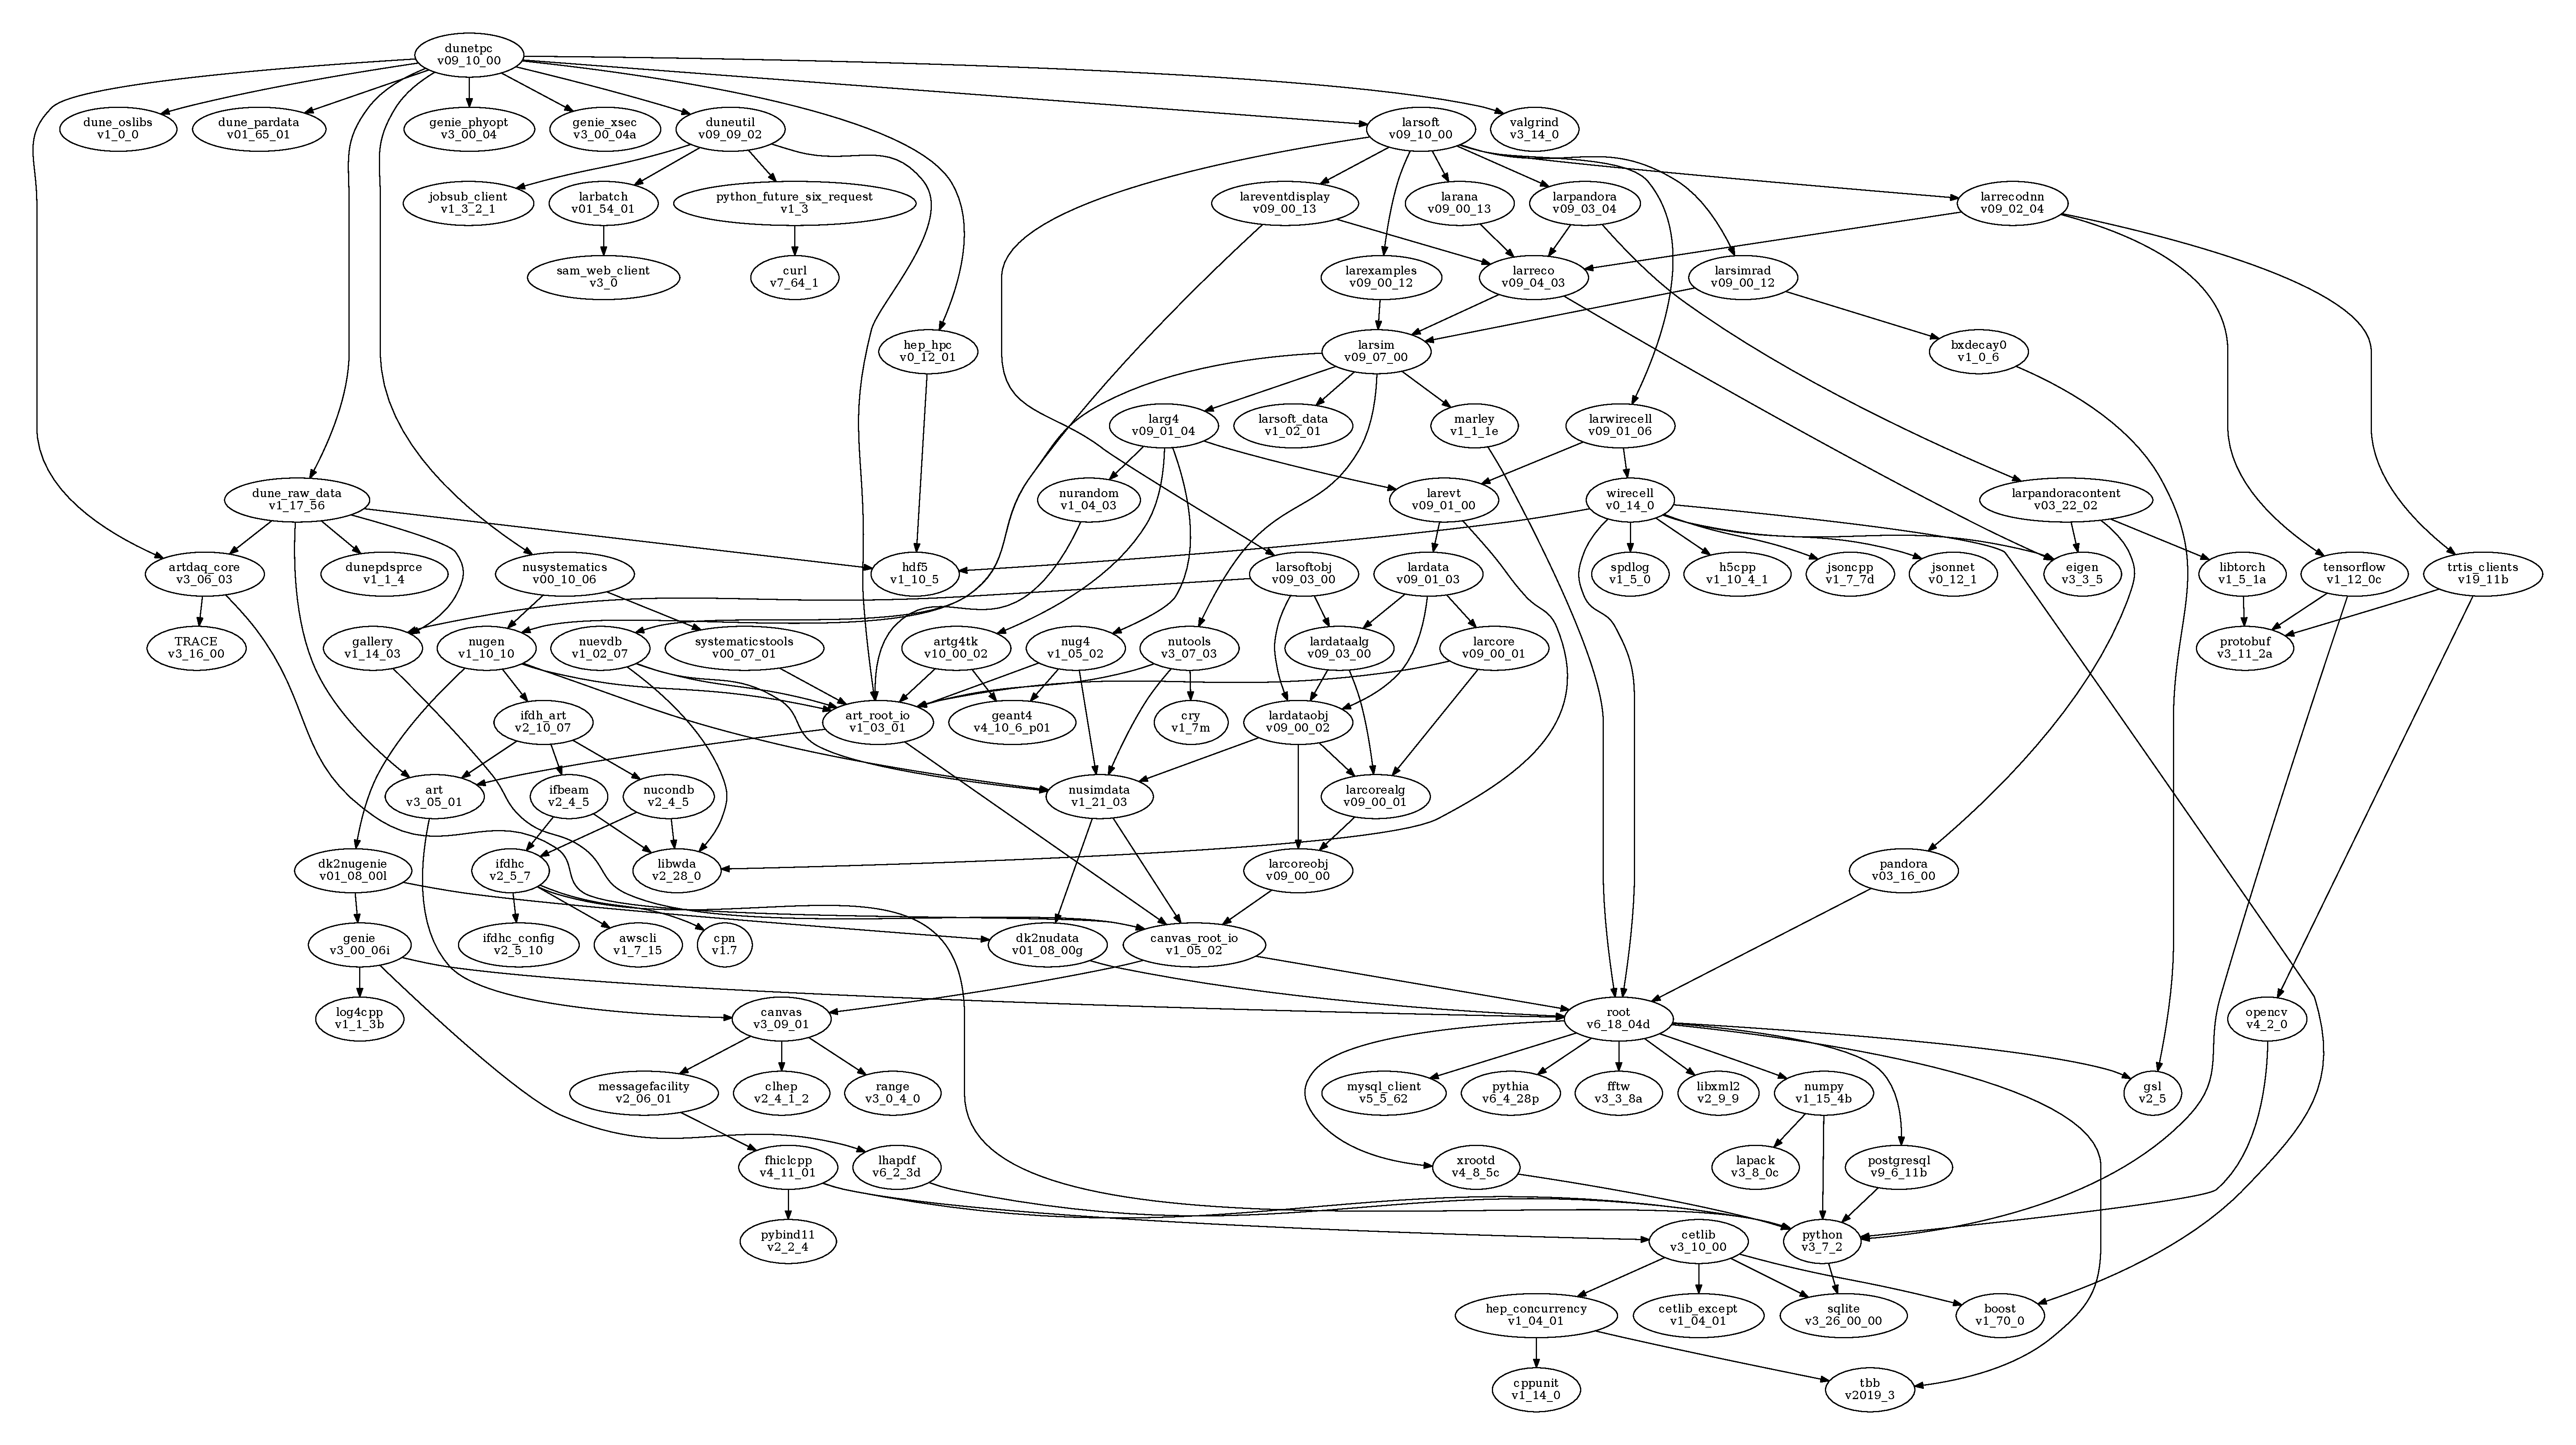
\includegraphics[width=\textwidth]{graphics/CodeManagementFigures/dunetpc_v09_10_00_depgraph.pdf}
\end{dunefigure}

LArSoft itself is split up into several repositories, such as larcore, larsim, larevt, lardata, and variations that have been split from them over time, such as lardataobj.  LArSoft is supported by Fermilab's Scientific Computing Division and is shared among several other experiments, such as ArgoNeuT, MicroBooNE, ICARUS and SBND.  The pool of developers is quite large, and the rate at which new code is added is quite significant.  New releases of LArSoft are made weekly.  Since dunetpc depends on LArSoft and sets it up via UPS, dunetpc also has a weekly release schedule.  LArSoft's repositories had been hosted in Fermilab's Redmine instance until 2018, at which point they were migrated to GitHub, and at the same time, a pull-request model was instituted, which enforces review of each commit before it is merged.  As of this writing, the dunetpc git repository is maintained in Fermilab's Redmine instance still allows commits from a large list of developers directly into the develop branch.  Following LArSoft's example of splitting it up into smaller pieces, migrating to GitHub, and adopting a pull-request model are on the list of to-do items.

The build system used is {\tt mrb}, which is provided by and supported by Fermilab's SDC.  Software is built in UPS products which are distributed to the collaboration in two ways.  The primary distribution mechanism is via a set of installed products in CVMFS which can be directly set up by end users without the need to install anything locally.  CVMFS maintains a cache on the user's computer to store copies of the released software files for repeated local access.  CVMFS is also used to distribute released software to batch worker nodes.  The second software mechanism is via the scisoft.fnal.gov web server.  UPS products are tarred up and the tarballs are uploaded to the scisoft web server, along with a manifest file which describes which tarballs need to be downloaded and installed to get a full, runnable dunetpc software stack.

In addition to code, some data files also are distributed via CVMFS.  For example, photon lookup libraries are stored in several-hundred-megabyte rootfiles which are inconvenient to store in a git repository.  They are loaded into a special repository in CVMFS and scisoft called dune\_pardata.  Even larger files are stored in StashCache which has a CVMFS interface for the user, but which retrieves files out of a dedicated area in dCache.

We are evaluating Spack as a replacement for {\tt mrb} and UPS.  Spack is a build system that also allows users to select from a list of installed versions, like UPS.  As operating systems become more secure, some of the ways of distributing, setting up, and running HEP software have conflicted with security features of the operating systems.  One of these is the use of the symbol {\tt LD\_LIBRARY\_PATH}.  UPS uses {\tt LD\_LIBRARY\_PATH} to point a user's environment at directories that contain the versions of released products that can be loaded and run.  Changing the contents of the {\tt LD\_LIBRARY\_PATH} variable causes the same program to load different versions of libraries.  Proper use of UPS maintains compatibility.  However, with newer operating systems, the shared libraries that are linked with programs and other shared libraries must be in the same locations as they where when linked, and not relocated.  The library that links to another keeps track of the installed locations of the libraries it links with.  Alternatively, the paths in which the dependent libraries are found can be edited after installation, in effect re-performing a stage of the linking step.  Spack is aware of this and inserts the proper {\tt rpath} values into linked libraries.

The use of Spack is under evaluation.  UPS is now approximately 25 years old and it is not an industry standard, somewhat linked to Fermilab.  Spack has a significant community using it outside of HEP, and thus there is a large volume of documentation available for it on the web.

%%%%%%%%%%%%%%%%%%%%%%%%%%%%%%%%
\section{Near Detector Code Management \hideme{Muether/Cremonisi/Junk needs update}}
\label{sec:codemgmt:neardet}  %% fix label according to section


\begin{dunefigure}
[Dependency graph for the GArSoft software stack. Nov 2020]
{fig:garsoftdeptree}
{Dependency graph for the GArSoft software stack, for version v02\_08\_00, November 2020.}
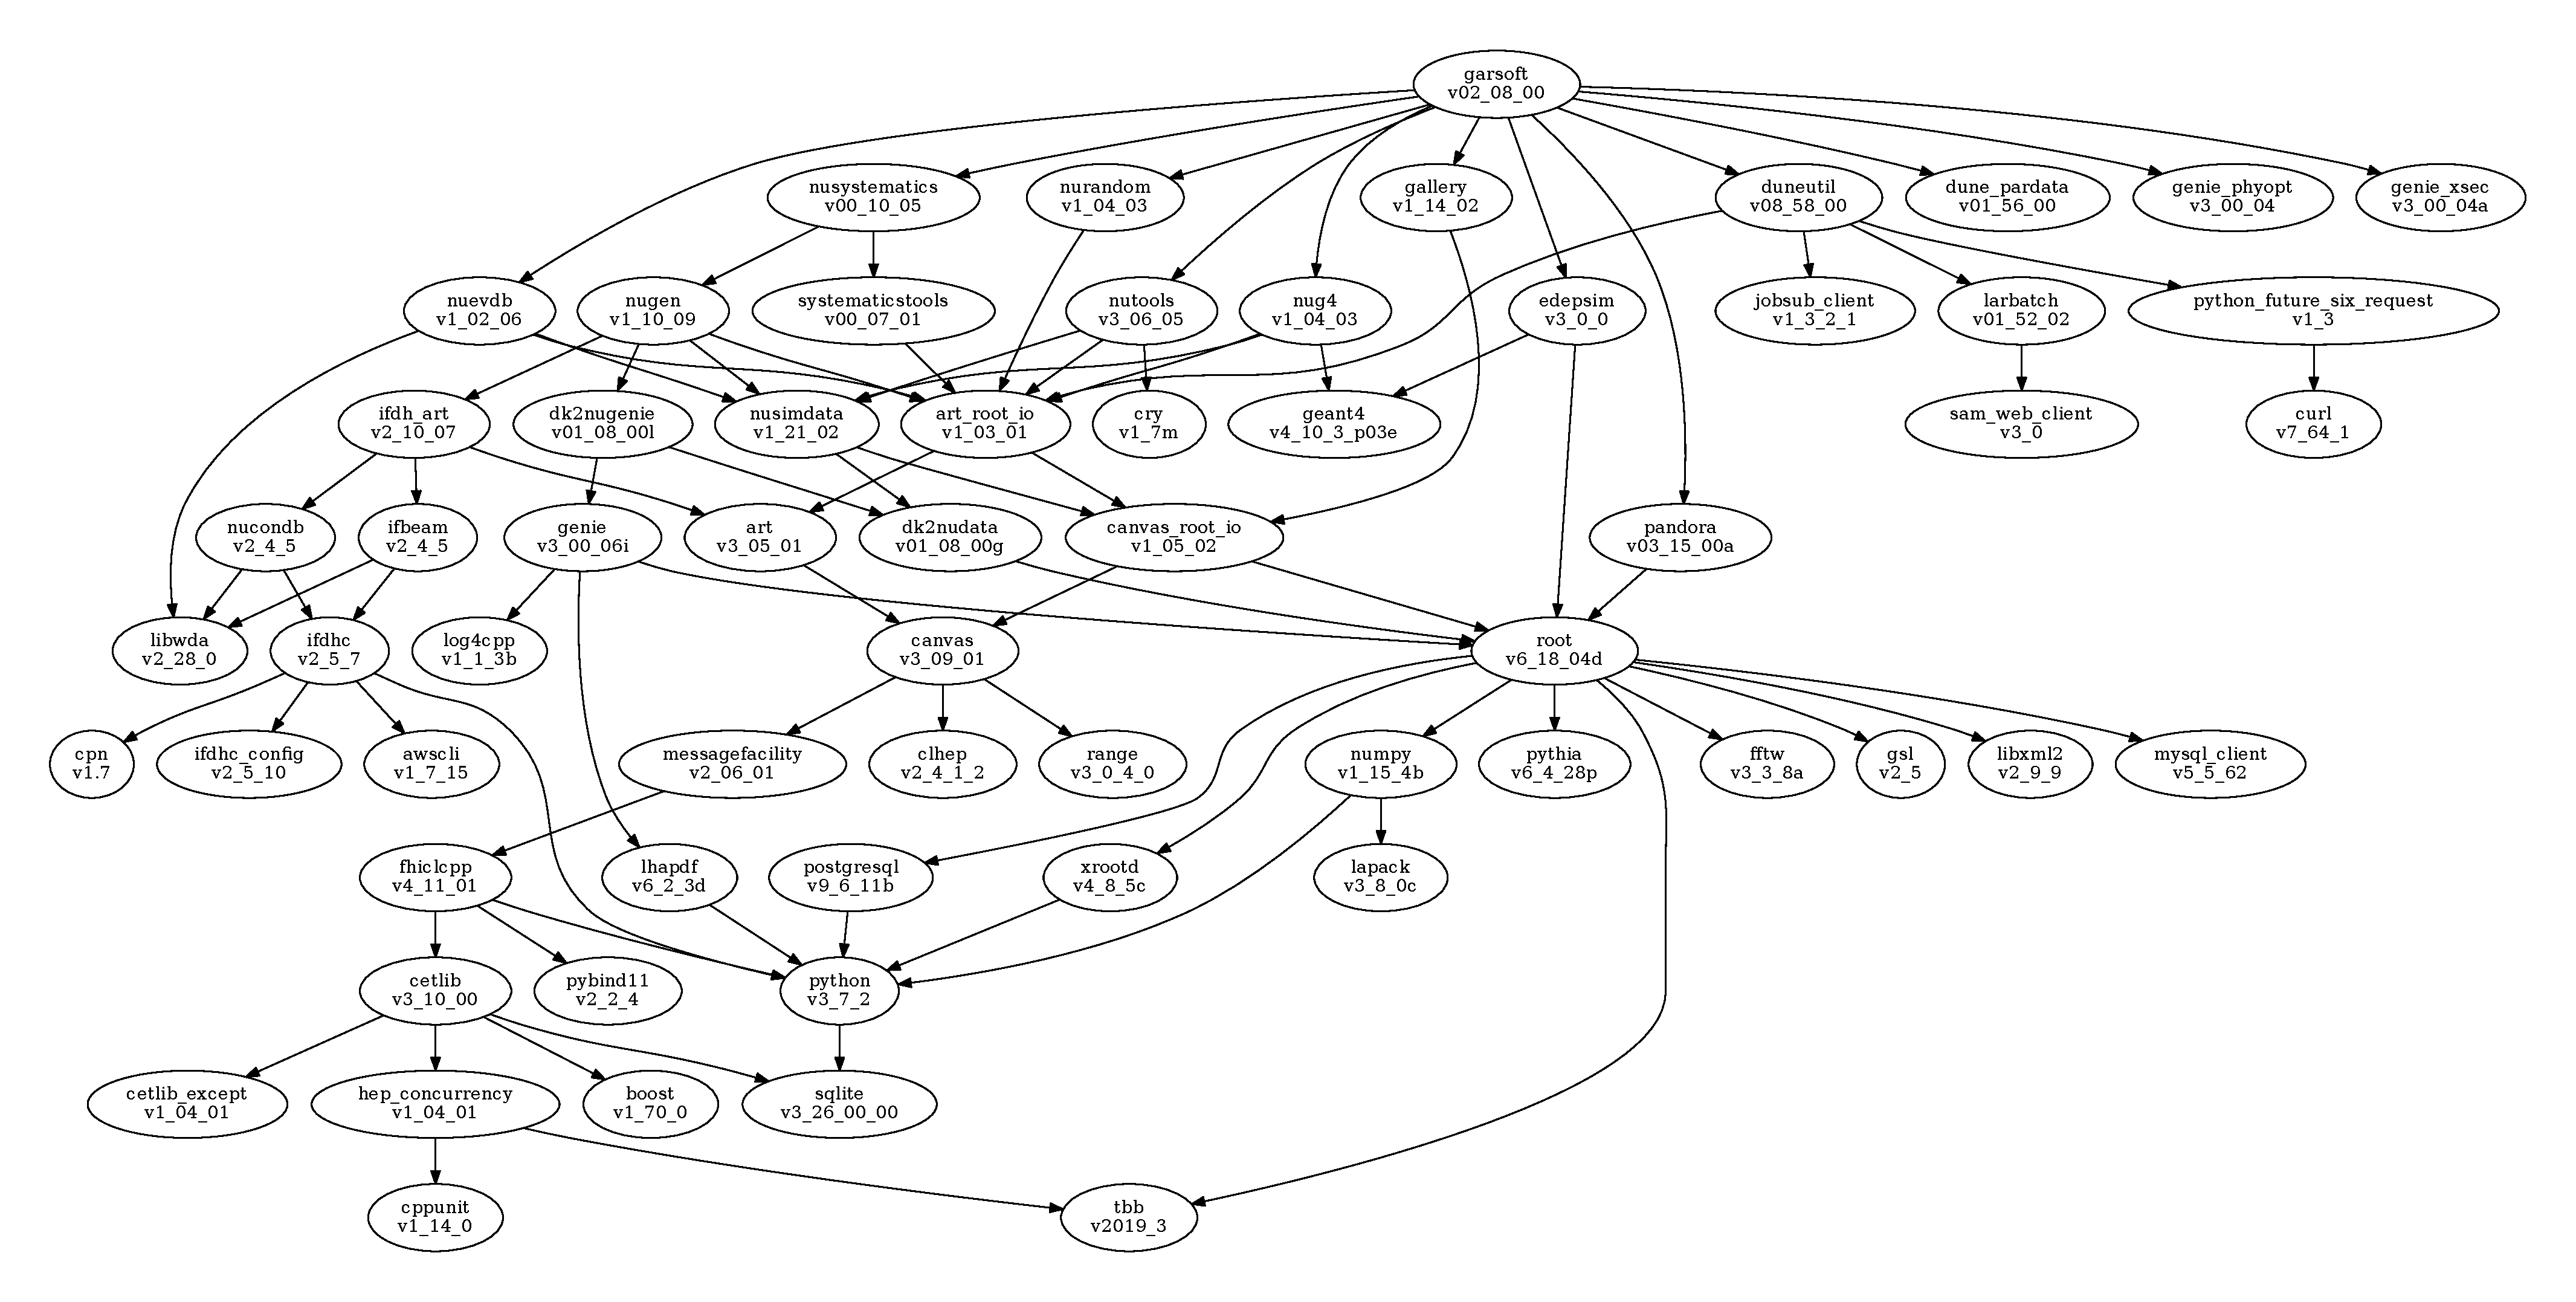
\includegraphics[width=\textwidth]{graphics/CodeManagementFigures/garsoft_v02_08_00_depgraph.pdf}
\end{dunefigure}

\section{Continuous Integration \hideme{Junk - draft}}
\label{sec:codemgmt:ci}

The stability of the performance of a large base of shared software requires attention to each change that is committed.  Software releases require validation and approval before being used in analyses intended for publication.  The rapid pace of software development early in the life cycle of the experiment, as well as increased activity as data are first collected and conferences come up, requires constant vigilance to ensure that bugs are not introduced and that software remains backwards compatible.

To meet this requirement, an automated continuous integration (CI) system is currently in operation for the LArSoft-based code base.  Similar systems, even using the same infrastructure, will be deployed for the near detector and beam simulations system.  The CI system consists of a set of servers that monitor commits pushed to the central code repositories.  On each commit, with a suitable delay of approximately 15 minutes in order to aggregate commits.  The CI system can also be triggered by user interaction, via an authenticated request.

Once triggered, the CI system will compile the changed code as well as any dependencies that are required.  Currently, the CI system builds LArSoft and all experiment code from the head of the develop branch in the repositories.  This is done because new commits to one repository, be it experiment-specific code or shared LArSoft code, may depend on the latest version of software in other repositories.  If shared software is the subject of the commit, then software that depends on it, such as all the experiment software stacks, are rebuilt, as a change to a header file in a shared repository can cause any source file that includes it, even indirectly, to fail to build.

The status of the build is stored in a logfile and summarized on a web page.  If a commit causes the build to fail, software managers and the person who committed and/or pushed the commit are notified and the commit is blocked from being merged into the head of develop.  LArSoft currently implements a pull-request model, in which experiment-appointed Level-2 managers comment on and sign off on changes to the central code, and Level-1 managers perform the actual merging.  A proposed change will not even be sent out for approval unless the CI system can build it and validation tests are run to compare output that ought not to have been changed by the new code.

This second step, physics performance validation, requires a more lengthy run through both unit tests and integration tests that run simulation and reconstruction workflows.  These tests run on standard input files and have their random number seeds fixed to constants.  The outputs are compared with reference histograms and a web page summarizes the comparison of the output logfiles, histograms, as well as run times and memory consumption, all of which are available on a web site that monitors these tests.  History plots of variables such as run time and memory consumption are made available on the monitoring web site so that investigations of when the memory usage of a job jumped up can be done without laborously checking out, building, and running the software in the suspected timeframe looking for a particular change.
\end{document}
